% Main file for libamtrack manual
% Copyright 2006, 2010 Steffen Greilich / the libamtrack team
% This file is part of the libAmTrack project (libamtrack.dkfz.org).

\documentclass[10pt,a4paper]{book}

\usepackage{amssymb}
\usepackage{amsmath}
\usepackage{array}
\usepackage[version=3]{mhchem}
\usepackage{lineno}
\usepackage{tensor}
\usepackage{graphicx}

% include hyperlinks in document and gives the pdf a title
\usepackage[pdftitle={libAmTrack Manual}]{hyperref}

\newcommand{\la}{\texttt{libAmTrack}}



\title{\la{} Manual}
\author{Steffen Greilich / the \la{} team}
\date{\today}


\begin{document}

\maketitle

\tableofcontents

% File for libamtrack manual
% Copyright 2006, 2010 Steffen Greilich / the libamtrack team
% This file is part of the libAmTrack project (libamtrack.dkfz.org).

\chapter{Introduction}

\la{} is a library of computational routines for the prediction of solid state detector response and radiobiological effectiveness in proton and ion beams. In this field, \la{} focusses on methods that are based on widely used amorphous track models (ATMs) rather than for example microdosimetry models.

Direct comparisons between ATMs are usually hampered by the lack of knowledge on the details of the modelling and computational procedures. We believe that this hinders a wider application of ATMs and the advance towards a better accurracy of their predictions. 

The \la{} project has therefore been started with the intention to provide an open-source, freely available, and comprehensive code for the community. Written in ANSI C, it is designed to be used independent of which platform the user is working on. Furthermore, the idea behind organizing \la{} as a library is that the user can access its functionality from whatever software tools they are using, e.g. MatLab, R, S-Plus etc.

The organization and documentation of the code -- albeit still far from being perfect -- should help to use \la{} for educational purposes as well.


\section{Amorphous track models}

ATMs (slightly confusing also referred to as 'track structure models') disregard the stochastic energy deposition pattern by secondary electrons around the track heavy charged particles (protons or ions, HCPs) considering only the averaged dose as a function of distance $r$ from the trajectory, i.e. the radial dose distribution $d(r)$ (\mbox{(FIGURE?)}). As photons deposit their energy eventually by electrons as well, local radiation effects are supposed to be the same. Thus, the detector response to irradiation with particles of type $T$ and energy $E$ can be predicted from the homogenous bulk photon dose response $S_X(D)$ of the detector system and the spatial deposition of local dose $d(x,y)$ as calculated from the fluences $\Phi(E, T)$ of the particle field. Despite many simplifications, ATMs are reasonably successful in predicting the response for a variety of physical detectors and biological systems \cite{Katz_et_al_1972, Waligorski_and_Katz_1980, Geiss_et_al_1997, Bassler_et_al_2008}. 


\section*{Document status}
\begin{tabular}{l l}
2010.05.28&Created by S. Greilich
\end{tabular}
% File for libamtrack manual
% Copyright 2006, 2010 Steffen Greilich / the libamtrack team
% This file is part of the libAmTrack project (libamtrack.dkfz.org).

\chapter{Installation}

The \la{} project is hosted at \texttt{libamtrack.sourceforge.net} using \texttt{svn} version control. Regularily, release versions are published.

\section{Installing GNU Scientific Library (GSL)}

A prerequsit for using \la{} is GSL (\texttt{http://www.gnu.org/software/gsl/}) as \la{} uses many of its numerical functions.

\begin{itemize}
\item{For most Linux distributions you can install GSL from repositories. Make sure that the GSL path is added to the library path. If you want to or have to compile \la{} yourself you will have to install the header files for GSL, too, i.e. the developer version.}
\item{For Windows there is a port available (\texttt{http://gnuwin32.sourceforge.net/packages/gsl.htm}). To work correctly, it is necessary that the binary files (\texttt{libgsl.dll} and \texttt{libgslcblas.dll}) are placed in the same directory as \texttt{libamtrack.dll}.}
\end{itemize}

\section{Installing \la{} binaries (for Windows only)}
The easiest way to get \la{} is to download the latest compiled version.

\section{Installing \la{} from latest released source code}

\section{Installing \la{} working version}

\subsection{Using Eclipse IDK}

\subsection{Using gcc only}



\section*{Document status}
\begin{tabular}{l l}
2010.05.28&Created by S. Greilich
\end{tabular}
% File for libamtrack manual
% Copyright 2006, 2010 Steffen Greilich / the libamtrack team
% This file is part of the libAmTrack project (libamtrack.dkfz.org).

\chapter{\la{} methods}

\section{Introduction}
'Methods' are the top-level routines in \la{}. From the physical parameters describing a HCP field they compute the predicted RE or RBE. In order to do so, the user has to both chose 
\begin{itemize}
\item{method independent settings, such as the radiation field, RDD, ER, gamma model and}
\item{method specific setting, e.g. the binning width to be used.}
\end{itemize}

Methods are implemented in the \texttt{Amtrack.c} and make use of all other subordinate routines. At the moment, four methods are available, Tab. \ref{tbl:Methods} gives an overview. All 	methods apply to slice of a homogenous detector being infinitesimally small in $z$ direction\footnote{Or a slice of the detector with finite size in $z$ but with crucial parameters, such as LET, fluence etc. not changing significantly over $\Delta z$}, i.e. in direction of the beam. The latter is supposed to be perfectly parallel and homogenous in fluence with respect to $x$ and $y$ (Fig. \ref{fig:Coordinates}. 

\begin{figure*}
	\centering
		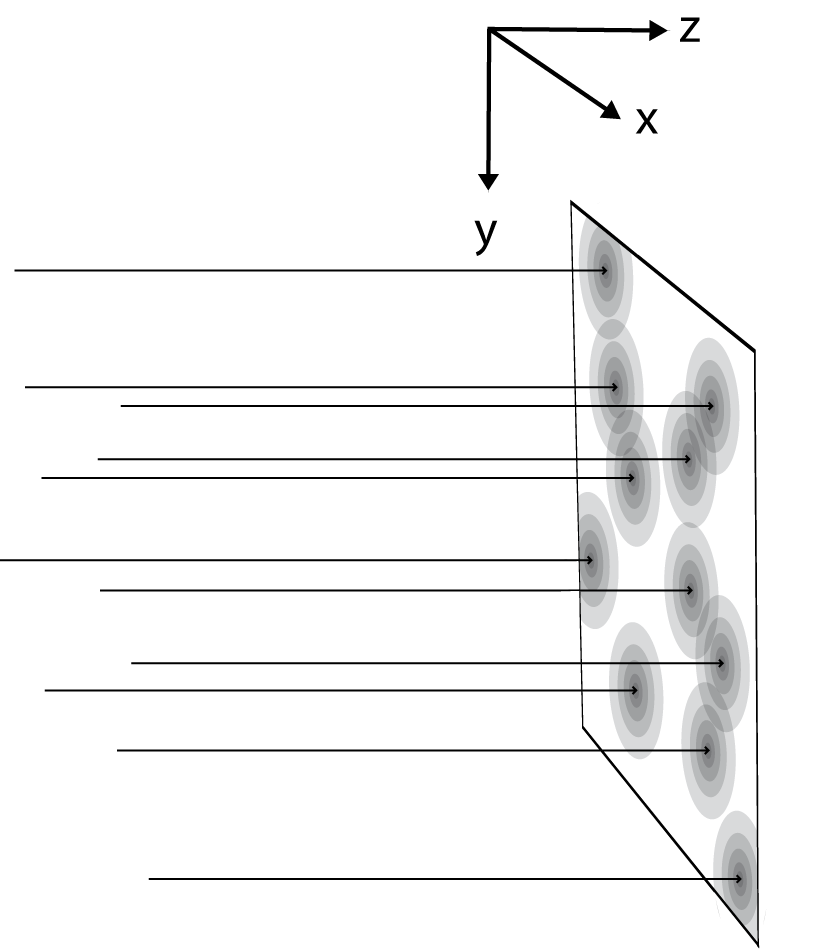
\includegraphics[bb=0 0 839 952,width=0.5\textwidth]{pictures/CoordinatesMethods.png}
	\caption{Coordinate definition in \la{}}
	\label{fig:Coordinates}
\end{figure*}

All methods share the following input parameters:\\
\begin{tabular}{p{0.25\textwidth} p{0.75\textwidth}}
\texttt{n} & number of components in mixed field (long integer) \\
\texttt{E\_MeV\_u[]} & the kinetic energy per nucleon for each component (array of double, size \texttt{n}) \\
\texttt{particle\_no[]} & the particle id number for each component, see ref. for more details (array of long, size \texttt{n}) \\
\texttt{fluence\_cm2[]} & the fluence (in cm$^{-2}$) or the dose (in Gy), if negative, for each component (array of double, size \texttt{n}) \\
\texttt{material\_no} & the material id number (long integer) \\
\texttt{rdd\_model} & the radial dose distribution id number, see \ref{chap:RDDs} for details (long) \\
\texttt{rdd\_parameters[]} & parameters for the given RDD, see \ref{chap:RDDs} for details (array of long, size depending on RDD model) \\
\texttt{er\_model} & the electron range id number, see \ref{chap:ERs} for details (long) \\
\texttt{gamma\_model} & the photon response id number, see \ref{chap:GRs} for details (long) \\
\texttt{gamma\_parameters[]} & parameters for the given RDD, see \ref{chap:GRs} for details (array of long, size depending on GR model) \\
\end{tabular}\\

All methods need in addition an array to return their results:\\
\begin{tabular}{p{0.25\textwidth} p{0.75\textwidth}}
\texttt{results[]} & the particle id number for each component (array of long, size 10) \\
\end{tabular}

\begin{table}
\label{tbl:Methods}
\begin{tabular}{m{0.25\textwidth}m{0.60\textwidth}m{0.15\textwidth}}

\hline
\textbf{Name} & \textbf{Description} & \textbf{Reference} \\
\hline

\begin{center}Ion-Gamma-Kill (IGK)\end{center}&
\footnotesize{Get activation cross-section by fusing photon response (activation probability) and RDD, get particle response by cross-section and fluence (ion-kill, intratrack action), for multi-hit systems and lower LET consider also intertrack action (gamma kill).}&
\begin{center}\cite{Waligorski_and_Katz_1980}\end{center}\\

\begin{center}Grid summation (GSM)\end{center}&
\footnotesize{,,Throw'' of particle tracks on a Cartesian grid for local dose, apply photon response for local response, then average response.}&
\begin{center}\cite{Geiss_et_al_1997}\end{center}\\

\begin{center}Compound Poisson processes using successive convolution (CPP-SC)\end{center}&
\footnotesize{Derive local dose frequency distribution analytically from RDD for single particle case, assume �none or one-impact situation for low fluence, convolute resulting distribution with itself until desired high fluence / dose is reached, apply photon response.}&
\begin{center}\cite{Greilich_et_al_CPPSC}\end{center}\\

\begin{center}Compound Poisson processes using statistical sampling (CPP-SS, SPISS)\end{center}&
\footnotesize{Derive local dose frequency distribution analytically from RDD for single particle case � as for CPPSC. But then use statistical sampling to add single impact doses according to relative fluences in the particle field.} &
\begin{center}\cite{Greilich_et_al_CPPSC}\end{center}\\

\hline
\end{tabular}
\caption{Methods implemented in \la{}.}
\end{table}


\section{The grid summation method (GSL)}
This is the most straight-forward approach: particles are sampled according to their relative fluence and local doses $d(x,y)$ --- and therefore local response $s(x,y)=S_X(d(x,y))$ --- are computed on a Cartesian grid ('checkerboard') by attributing the corresponding $d_{E,T}(r)$ to the sampled particle (FIGURE?). The detector is thought to be homogenous, perpendicular to the beam in $(x,y)$, and of negligible thickness $\Delta z$. The relative efficiency $\eta$ can then be estimated by averaging the local response $s$ over all grid elements:
\begin{equation}\label{eq:eta}
	\eta(\phi(E, T))=\frac{S_{HCP}}{S_X(D)}=\frac{\left\langle s\right\rangle}{S_X(\left\langle d\right\rangle)}
\end{equation}

Although conceptually straightforward, GSM can be very time-consuming, esp. in the case of higher fluences and particle energies (e.g. $E_{\mbox{proton}} >$ 20 MeV) with many contributions to a single voxel. Furthermore, the procedure has to be repeated many times in order to converge --- or a large detector grid has to be simulated. 


\section{The compount Poisson process methods (CPP)}

To overcome the limitations of GSM calculating the local dose distibution as a spatial deposition pattern $d(x,y)$, we consider a representative point $P$ (FIGURE?). The cumulative distribution function $F(d)$ of local dose $d$ in $P$ depends on the macroscopic fluence $\phi$ (and dose $D$, resp.) and the microscopic pattern around a track as expressed by $d(r)$. Then, one can state:
\begin{itemize}
	\item {$r_{max}$ is the maximum delta electron range in the field, so $P$ is only influenced by tracks within a circle $C$ of radius $r_{max}$ around $P$ (\mbox{FIGURE?}).}
	\item {All tracks in $C$ are contributing to $d$ and their number $n$ is Poisson distributed with mean $\mu=\phi\cdot\pi r_{max}^2$.}
	\item {Let $F_n$ be the cumulative distribution function of the local dose in the case of exactly $n$ tracks. For a single track traversing $C$, we readily have the cumulative single impact distribution
		\begin{equation}\label{eq:singletrack}
			F_1(d)=1-\frac{R(d)^2}{r_{max}^2},
		\end{equation}
		with $R(d)=D^{-1}(r)$ (\mbox{FIGURE?}).}
	\item {In the case of $n$ tracks in $C$, $d$ is the sum of $n$ independent and identically distributed single track doses, so $F_n$ can be expressed as the $n$-fold convolution of $F_1$:
		\begin{equation}\label{eq:ntracks}
			F_n=\underbrace{F_1*\ldots*F_1}_{\mbox{$n$ times}}
		\end{equation}
	}
	\item {As $n$ is Poisson distributed, $F$ is the distribution function of a compound Poisson process:
		\begin{equation}
			F(d)=e^{-\mu}\sum^{\infty}_{i=1}{\frac{\mu^i}{i!}F_i(d)}
		\end{equation}
	}
	\item {The derivative $f(d)$ of $F(d)$ can then be eventually used to compute the macroscopic HCP detector response as the expected local response $\left\langle s\right\rangle$:
		\begin{equation}
		  \langle s \rangle= \int_0^{\max(d)} S_X(d) f(d)\, \mathrm{d}d,
		\end{equation}
		and used in Eq. (\ref{eq:eta}) to get the $\eta$. A similar procedure for $\left\langle d\right\rangle$ provides a quality check as it has to meet $D$.
	}
\end{itemize}
This description enables $F$ to be determined from the explicitly given distribution function $F_1$ in the case of monoenergetic particle fields. It can easily be extended to mixed particle fields by using the adjusted $F_1$ from Eq.(\ref{eq:multitrack}) in Eq.(\ref{eq:ntracks}) with $p_{E,T}$ being the relative fluence and $R_{E,T}$ the inverse radial dose distribution for the composing particles
\begin{equation}\label{eq:multitrack}
  F_1(d)=1-\sum_{E,T}p_{E,T}\cdot\frac{R_{E,T}(d)^2}{\hat{r}_{max}^2},
\end{equation}
where $\hat{r}_{max}=max(r_{max}(E,T))$.

It should be stressed that the presented approach is in no way limited to handle extended targets despite the point nature of $P$ as the averaging across the target is already contained in $D(r)$ (for the difference between point and extended target distributions, see \cite{Katz_et_al_1972, Edmund_et_al_2007}). While the computation of detector response from the local dose distribution $F(d)$ is trivial, the numerical calculation of $F(d)$ itself can, however, be cumbersome. 



\subsection{Computation using statistical sampling (CPP-SS)}
One way to approximate $F(d)$ is the following:


The implementation of this approach in \la{} is named SPISS, which is explained below.



\subsection{Accelerated computation using successive convolution (CPP-SC)}
An approximation method for the rapid computation of compound Poisson processes was introduced by Kellerer \cite{Kellerer_1985}. It makes use of the fact that the distribution $f(d;\mu)$ can be obtained by a convolution operation:
	\begin{equation}
		f(d;\mu)=\int_{0}^{d}{f(d-t;\mu/2)\cdot f(t;\mu/2) dt}
	\end{equation}
One can chose a $\mu_{start}<<1$ with $\mu=2^m\cdot\mu_{start}$ so that multiple events can be neglected and therefore $f(d;\mu_{start})$ consists, in good approximation, of two components only, namely the probability of no track in $C$ ($d=0$) 
	\begin{equation}
		e^{-\mu_{start}}\approx (1-\mu_{start})=\hat{f}_0
	\end{equation}
and of the density related to a single track
	\begin{equation}
		\hat{f_1}\approx\mu_{start}\cdot f_1(d).
	\end{equation}
Performing $m$ successive convolutions on these two components, i.e. replacing
	\begin{equation}
		\hat{f}_0 \mbox{ by } \hat{f}_0^2
	\end{equation}
and
	\begin{equation}
		\hat{f}_1 \mbox{ by } 2\cdot\hat{f}_0\cdot\hat{f}_1 + \hat{f}_1*\hat{f}_1
	\end{equation}
will eventually yield $f(d)$. For obscure reasons, the implementation of this approach in \la{} is named CPPSC.




\section*{Document status}
\begin{tabular}{l l}
2010.05.28&Created by S. Greilich
\end{tabular}
\chapter{LEM description by Martin}

\section{Status of the document}

% File for libamtrack manual
% Copyright 2006, 2010 Steffen Greilich / the libamtrack team
% This file is part of the libAmTrack project (libamtrack.dkfz.org).

\chapter{Radial dose distributions}

One of the most disputed submodels in AT modelling is the parametrization of the distribution of radial dose around the particle tracks ('radial dose distribution', RDD). Up to now, \la{} can use the RDDs given in Tab. \ref{tbl:RDDs} and Fig. \ref{fig:RDDs}. 


\begin{table}
\label{tbl:RDDs}
\begin{tabular}{m{0.25\textwidth}m{0.60\textwidth}m{0.15\textwidth}}

\hline
\textbf{Name} & \textbf{Expression} & \textbf{Reference} \\
\hline

\begin{center}Test\end{center}&
$d(r)=c\cdot\Theta(-r_{max})$&
\textsl{simple step function}\\

\begin{center}Katz (point target)\end{center}&
$d(r)=\frac{N_e\cdot e^4}{m_e c^2}\cdot\frac{1}{{\rho}_m}\cdot\frac{z^2}{\beta^2}\cdot\frac{1}{\alpha}\cdot\frac{1}{r^2}\cdot (1-\frac{r}{r_{max}})^\alpha=d_{point}(r)$&\cite{Zhang_et_al_1985}\\

\begin{center}Katz (extended target)\end{center}&
$d(r)=\frac{1}{A}\int_{|r-a_0|}^{|r+a_0|}{2\cdot\Phi\cdot\hat{r}\cdot d_{point}(\hat{r})\cdot d\hat{r}}$&\cite{Waligorski_1988}\\

\begin{center}Site\end{center}&
$d(r)=\begin{cases}c&\text{if $r<a_0$,}\\
d_{point}(r)&\text{otherwise.}
\end{cases}$&\cite{Hansen_and_Olsen_1984}\\

\begin{center}Gei{\ss}\end{center}&
$d(r)=\begin{cases}c&\text{if $r<a_0$,}\\
\frac{c}{r^2}&\text{if $a0\le r\le r_{max}$}\\0&\text{if $r>r_{max}$}\end{cases}$&\cite{Geiss_et_al_1997}\\

\hline
\end{tabular}
\caption{RDDs implemented in \la{}.}
\end{table}


\begin{figure*}
	\centering
		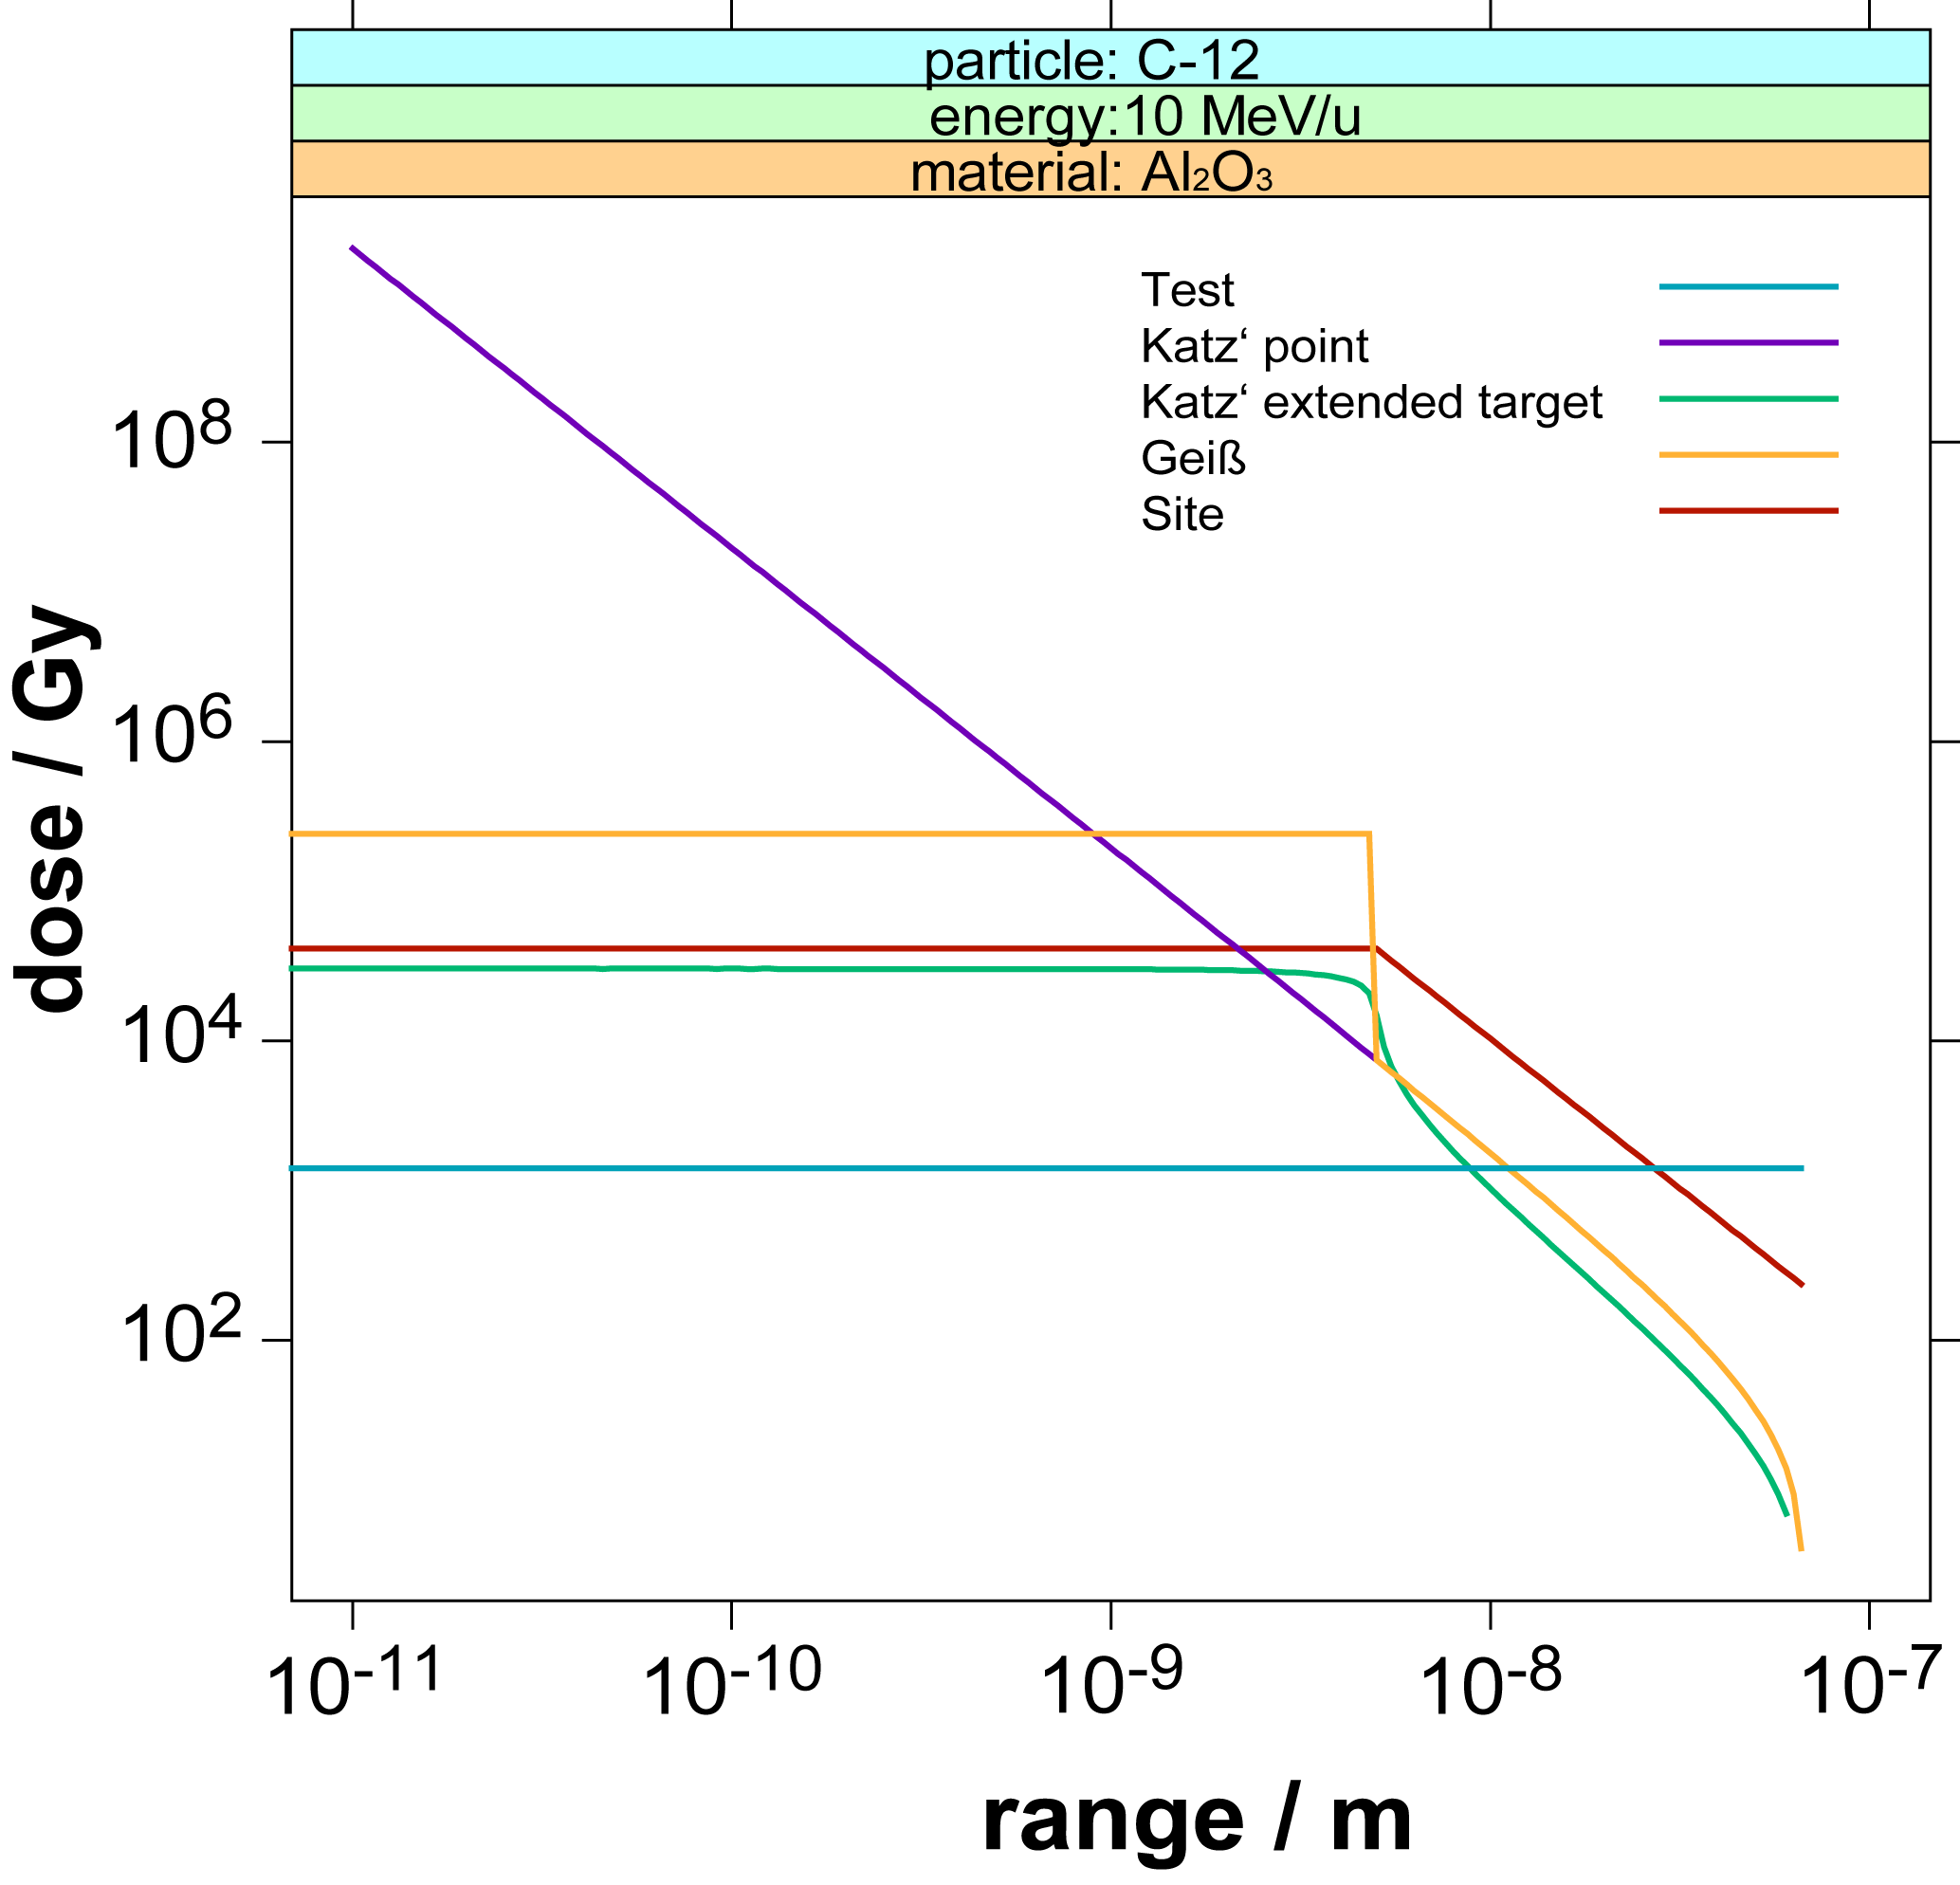
\includegraphics[width=1.0\textwidth]{RDD.png}
	\caption{Radial dose distribution submodels available in \la{}}
	\label{fig:RDDs}
\end{figure*}



\section*{Document status}
\begin{tabular}{l l}
2010.06.01&Created by S. Greilich
\end{tabular}
% File for libamtrack manual
% Copyright 2006, 2010 Steffen Greilich / the libamtrack team
% This file is part of the libAmTrack project (libamtrack.dkfz.org).

\chapter{Electron range relation}
\label{chap:ERs}

The submodels of electron-range relation determining the width of the particle tracks (Tab. \ref{tbl:ERs} and Fig. \ref{fig:ERs}) -- their differences can be up to two orders of magnitude at the upper end of the range of clinically used energies.


\begin{table}
\label{tbl:ERs}
\begin{tabular}{m{0.25\textwidth}p{0.60\textwidth}m{0.15\textwidth}}

\hline
\textbf{Name} & \textbf{Expression} & \textbf{Reference} \\
\hline

\begin{center}Butts and Katz\end{center}&
$r_{max}/\text{(g$\cdot$cm$^{-2}$)}=10^{-6}\cdot w/\text{keV} \text{   , with   } w/\text{keV}=2\cdot m_e\cdot ((\frac{E}{E_0})^2+2(\frac{E}{E_0})$
&\cite{Butts_and_Katz_1967}\\

\begin{center}Walig\'orski\end{center}&
$r_{max}/\text{(g$\cdot$cm$^{-2}$)}=6\cdot 10^{-6}\cdot (w/\text{keV})^\alpha \text{   , with   } \alpha=1.079(w<1\text{ keV) or } 1.667\text{ (otherwise)}$
&\cite{Waligorski_et_al_1986}\\

\begin{center}Geiss\end{center}&
$r_{max}/\text{cm}=4\cdot 10^{-5}\cdot (E/\text{MeV})^{1.5}\cdot \frac{\rho_{material}}{\rho_{water}}$
&\cite{Geiss_1998}\\

\begin{center}Scholz\end{center}&
$r_{max}/\text{$\mu$m}=0.05\cdot 10^{-5}\cdot (E/\text{MeV})^{1.7}\cdot \frac{\rho_{material}}{\rho_{water}}$
&\cite{Scholz_2001}\\

\hline
\end{tabular}
\caption{ERs implemented in \la{}.}
\end{table}


\begin{figure*}
	\centering
		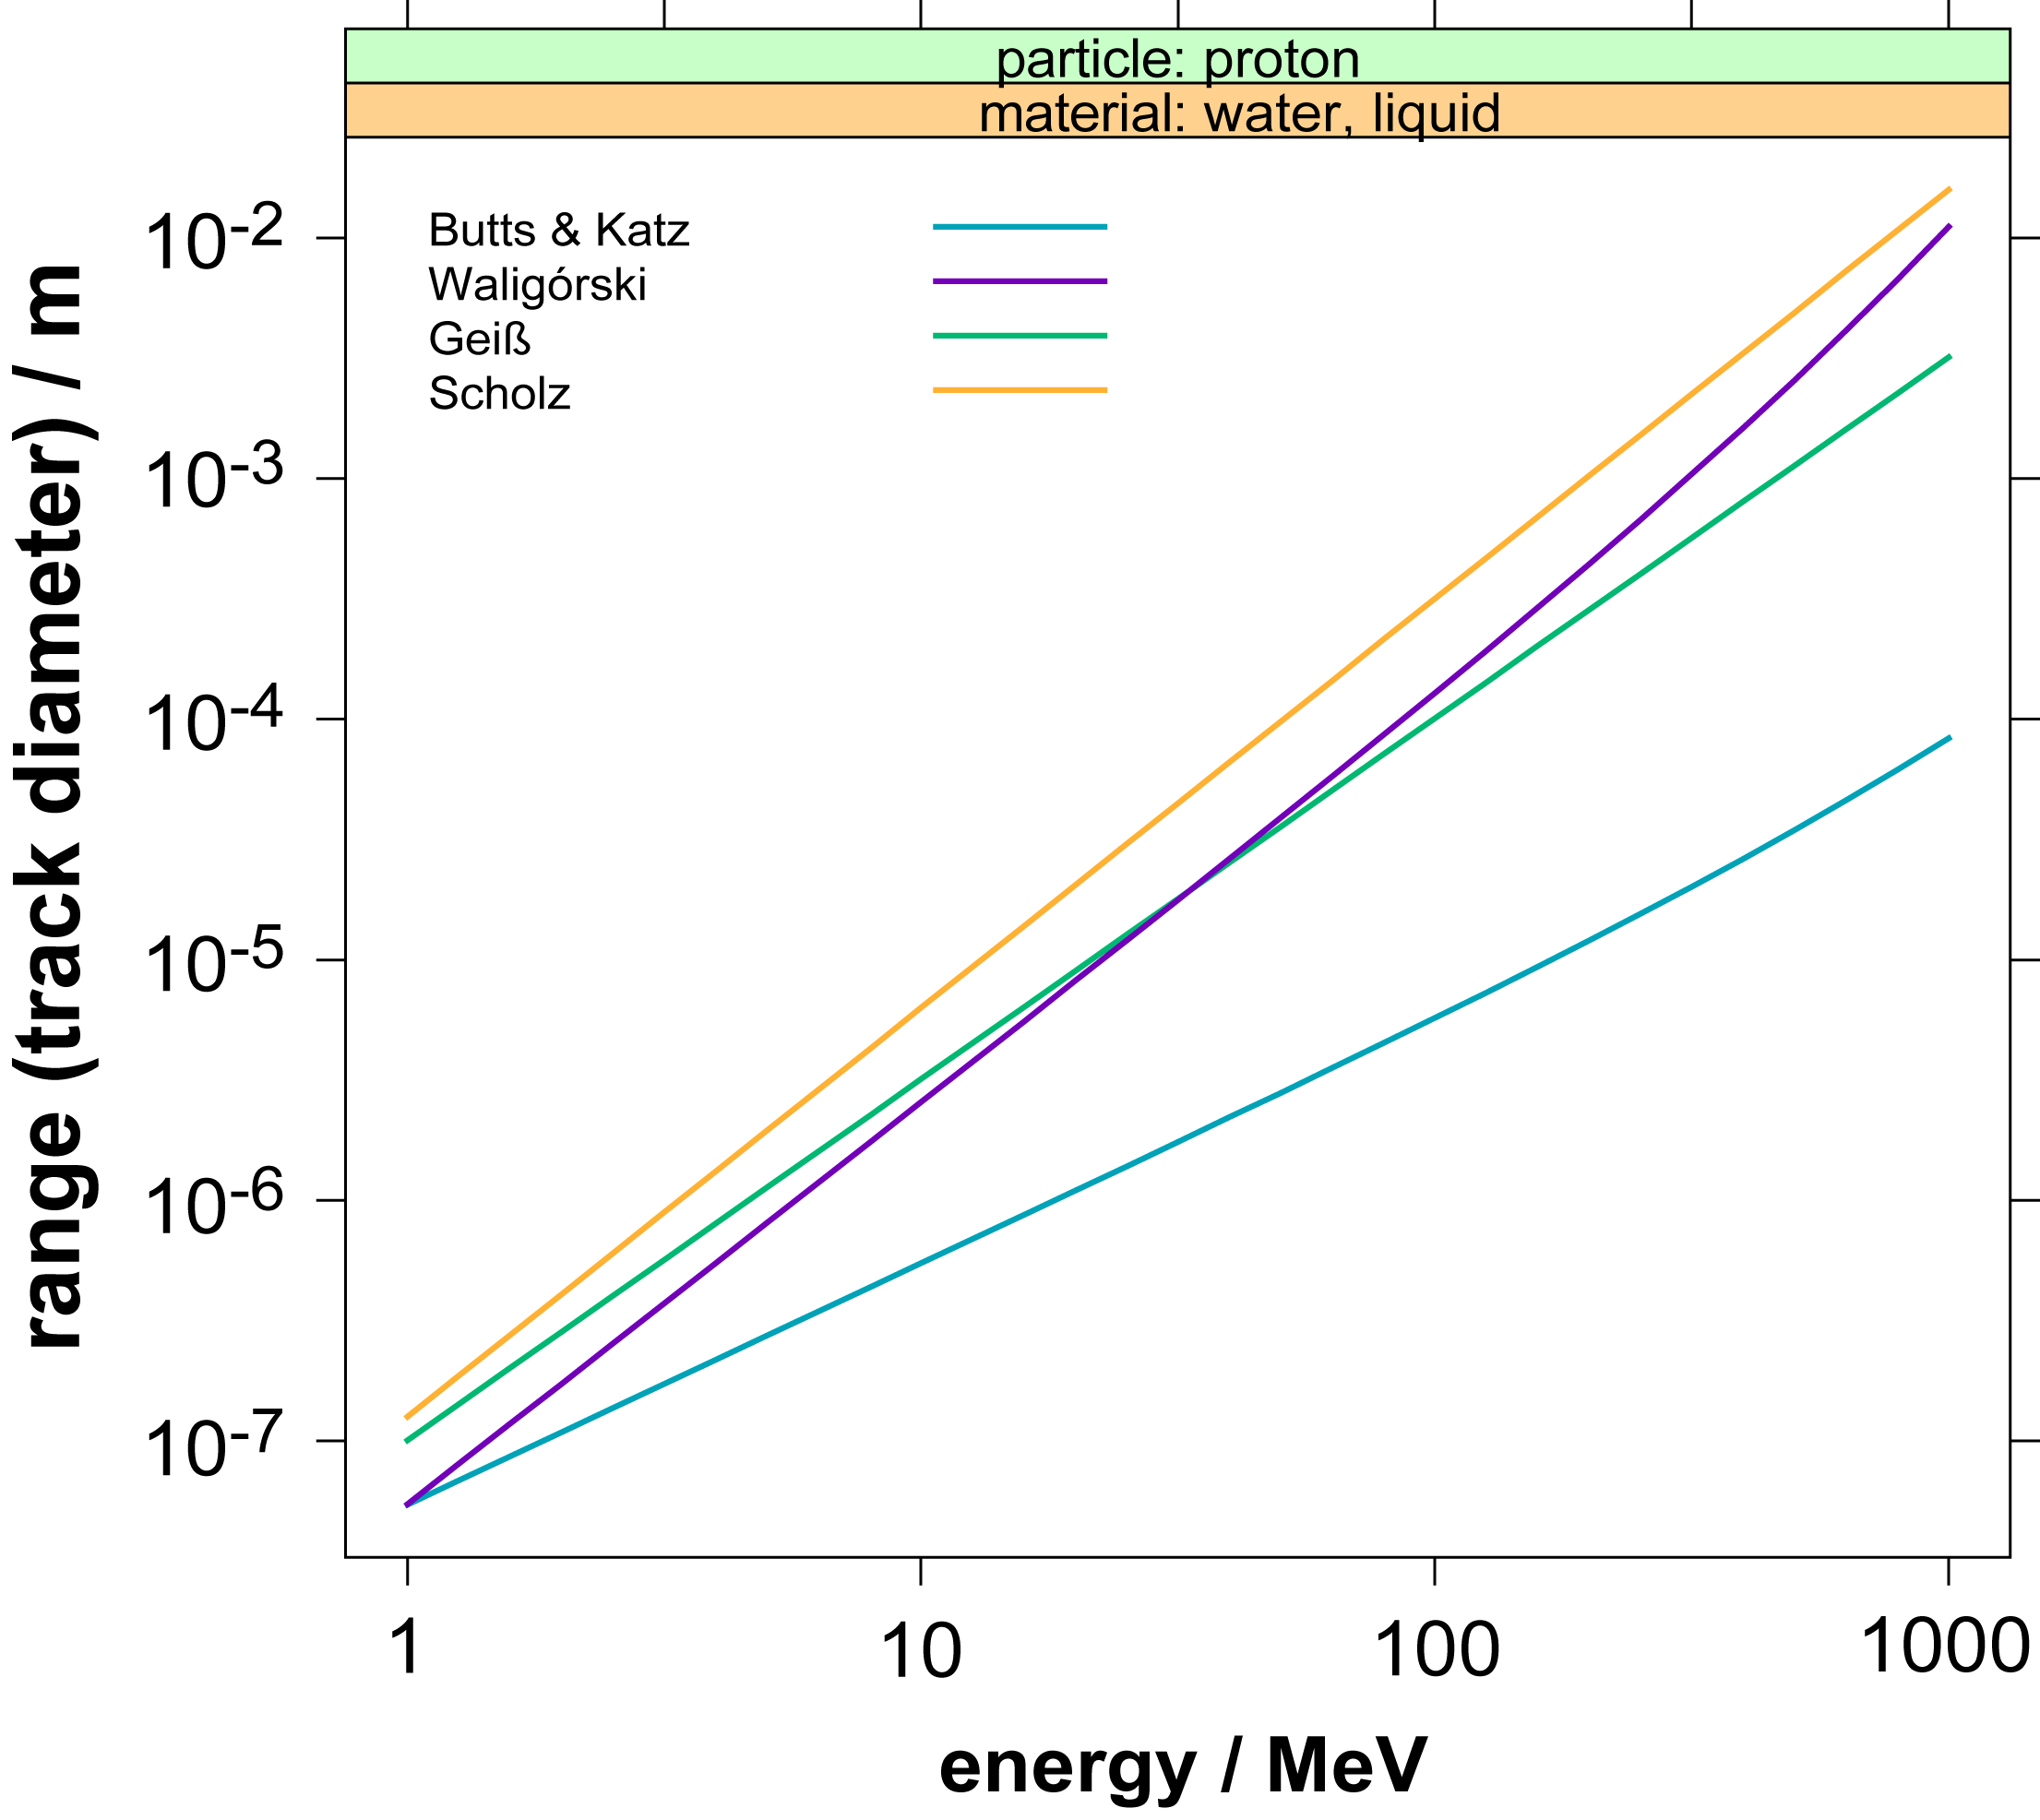
\includegraphics[bb=0 0 2211 1973,width=1.0\textwidth]{pictures/ER.png}
	\caption{Electron-range submodels available in \la{}.}
	\label{fig:ERs}
\end{figure*}


\section*{Document status}
\begin{tabular}{l l}
2010.06.01&Created by S. Greilich
\end{tabular}
% File for libamtrack manual
% Copyright 2006, 2010 Steffen Greilich / the libamtrack team
% This file is part of the libAmTrack project (libamtrack.dkfz.org).

\chapter{Photon response models}
\label{chap:GRs}

For the actual computation of HCP response, several photon-response relations are found in libamtrack (Tab. \ref{tbl:GRs} and and Fig. \ref{fig:GRs}). Again, they can almost freely combined with the ATMs (an important exception still being IGK which is bound to a general hit/target response).


\begin{table}
\label{tbl:table4}
\begin{tabular}{m{0.25\textwidth}p{0.60\textwidth}m{0.15\textwidth}}

\hline
\textbf{Name} & \textbf{Expression} & \textbf{Reference} \\
\hline

\begin{center}Test\end{center}&
$S(D)=a\cdot D+b$&
\textsl{simple linear function}\\

\begin{center}General hit/target\end{center}&
$S(D)=(1-sum_{k=0}^{c-1}{\frac{(D/D_0)^k}{k!}\cdot e^{-(D/D_0)}})^m$
&\cite{Dertinger_and_Jung_1970}\\

\begin{center}Radioluminescence\end{center}&
$S(D)=\begin{cases}c_1\cdot D+c_2 \cdot D^2&\text{if $D<D_{sat}$,}\\
c_3+c_4 \cdot D&\text{if $D\ge D_{sat}$,}
\end{cases}$&\cite{Andersen_et_al_2006}, \cite{Greilich_et_al_2008}\\

\begin{center}Exp.-saturation\end{center}&
$S(D)=c\cdot (1-e^{-D/D_0})$
&\textsl{simplified case of the general hit/target model}\\

\begin{center}Linear-quadratic\end{center}&
$S(D)=e^{-\alpha\cdot D-\beta \cdot D^2}$
&\cite{Chadwick_and_Leenhouts_1973}\\

\hline
\end{tabular}
\caption{Photons response models implemented in \la{}.}
\end{table}


\begin{figure*}
	\centering
		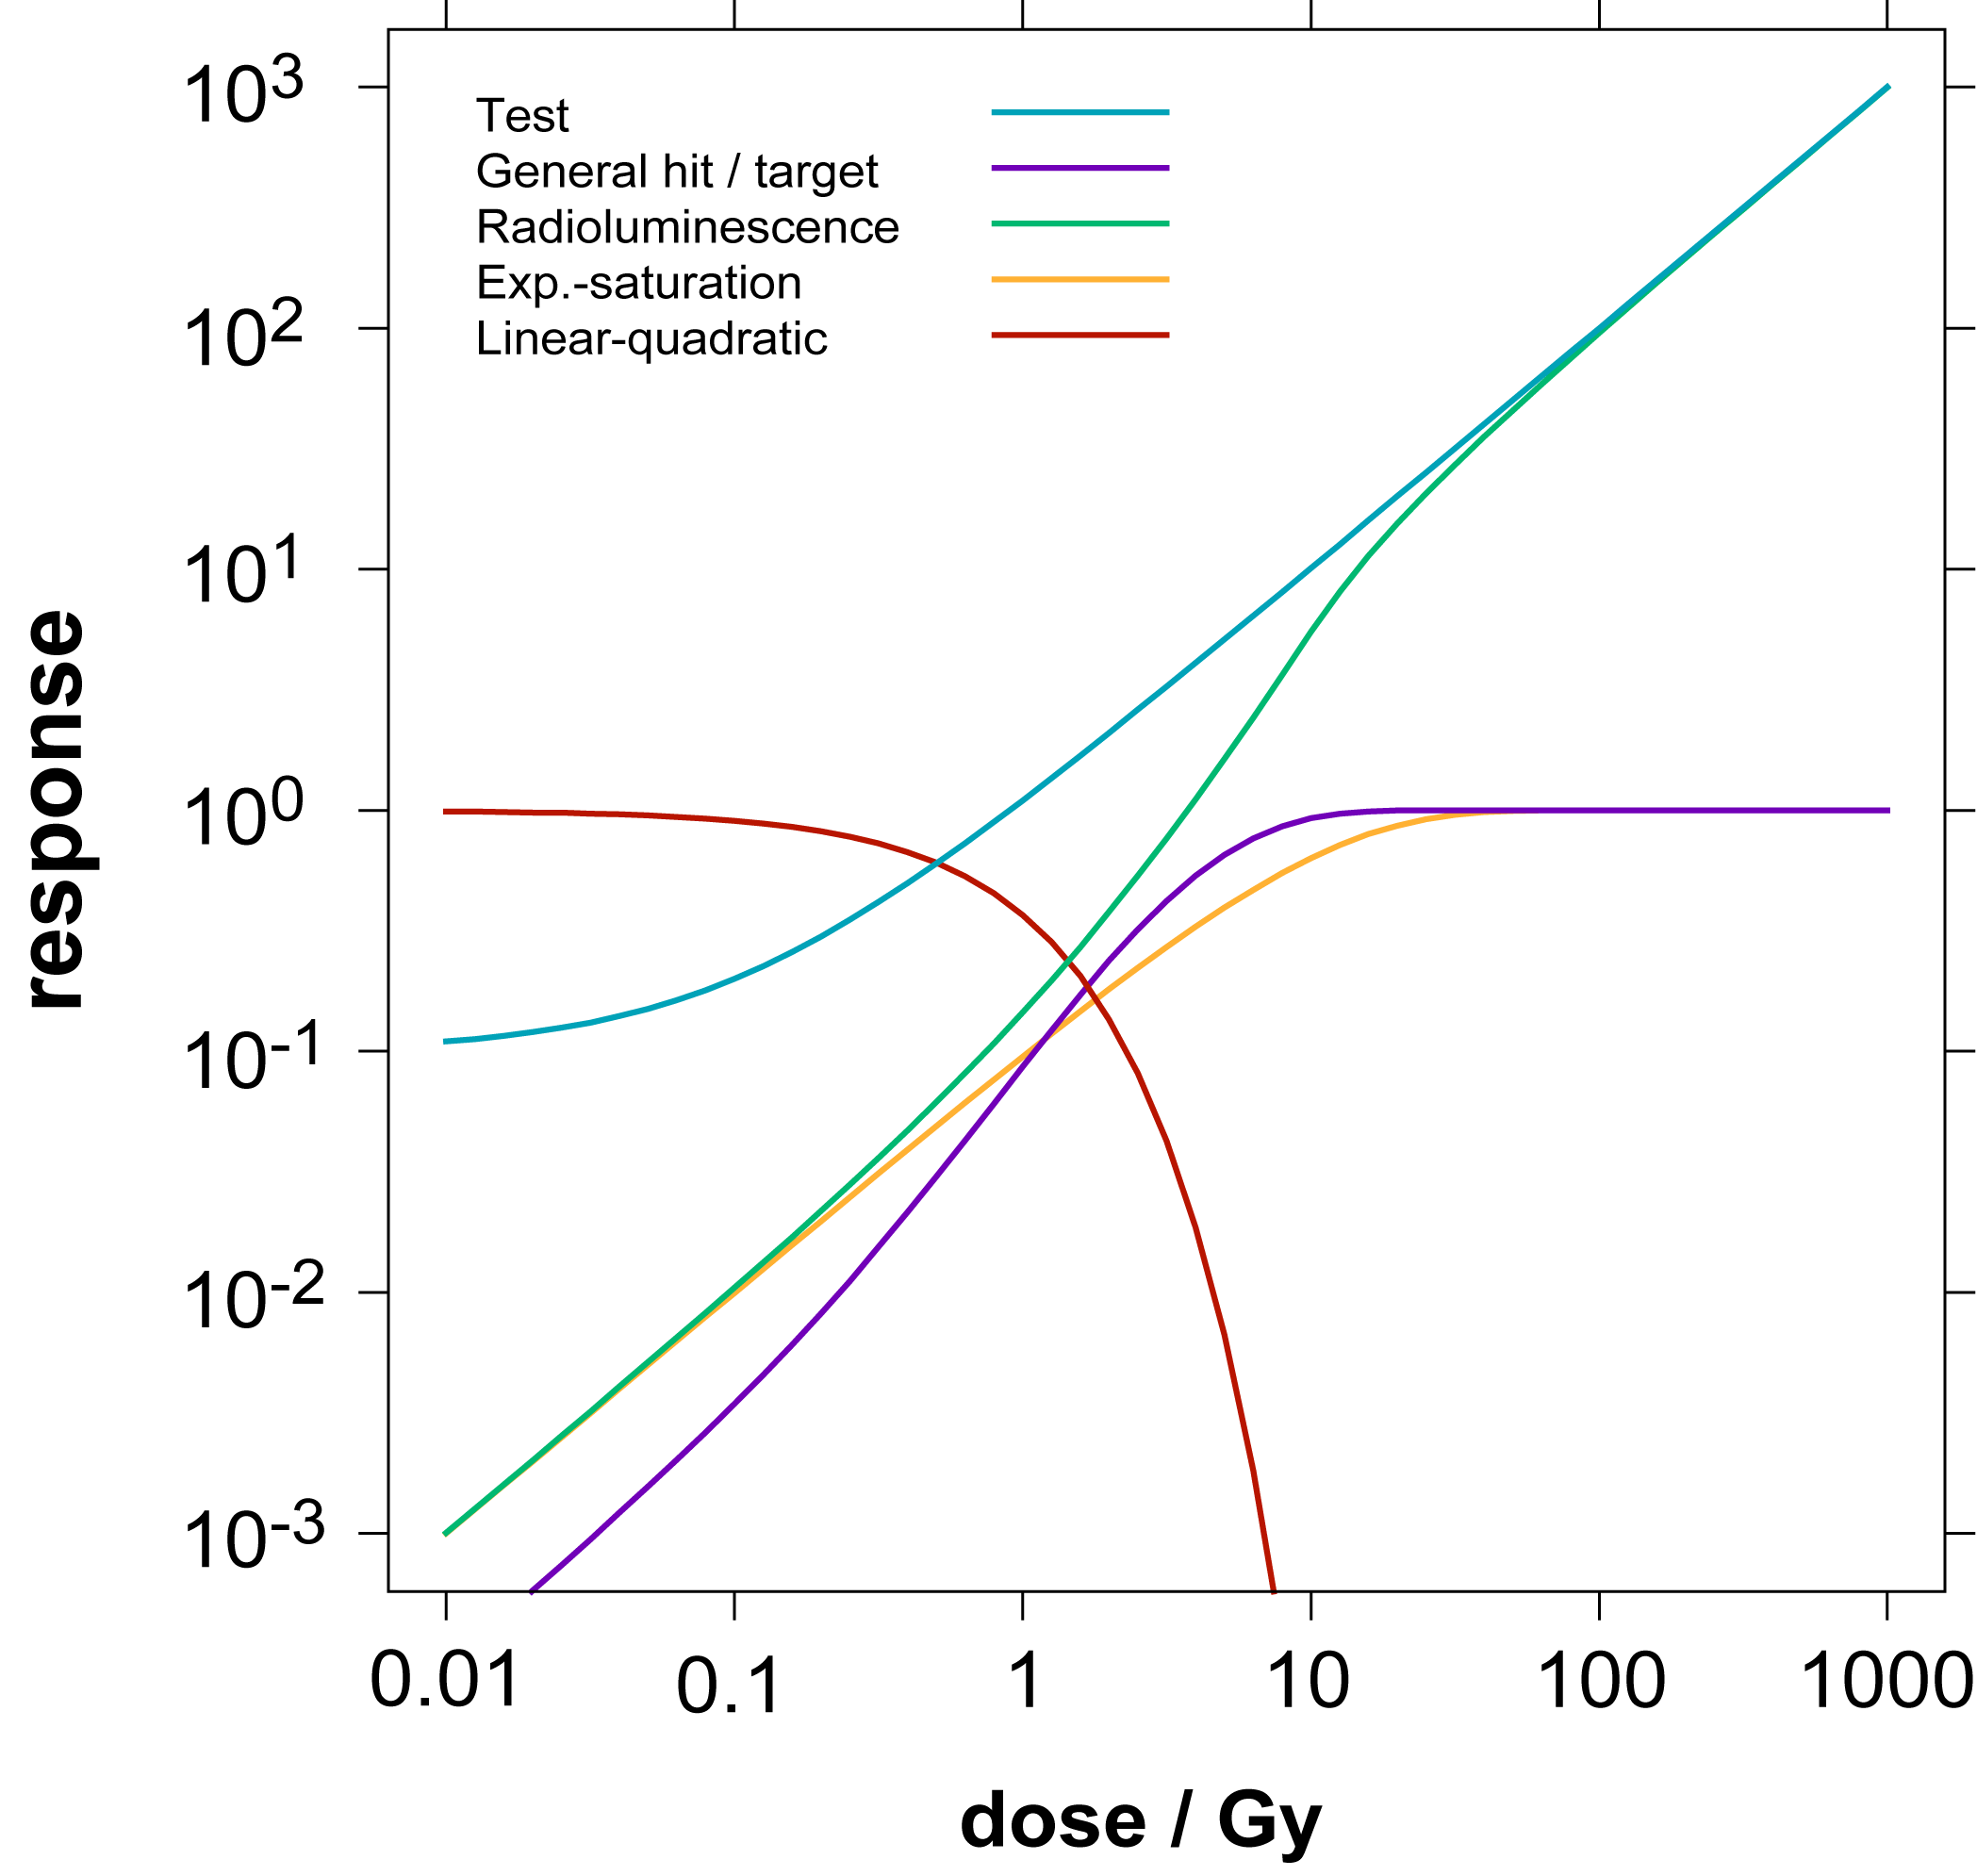
\includegraphics[width=1.0\textwidth]{pictures/GR.png}
	\caption{Photon-responses available in \la{}.}
	\label{fig:GRs}
\end{figure*}


\section*{Document status}
\begin{tabular}{l l}
2010.06.01&Created by S. Greilich
\end{tabular}
% File for libamtrack manual
% Copyright 2006, 2010 Steffen Greilich / the libamtrack team
% This file is part of the libAmTrack project (libamtrack.dkfz.org).

\chapter{Physics routines}

\texttt{libamtrack} contains a number of auxiliary routines handling the physics of ion beams needed. These routines can be used independently from the efficiency methods. They are implemented in \texttt{AT\_PhysicsRoutines.c} and are described in detail in this.

\section{\texttt{AT\_beta\_from\_E}}

Computes the relativistic speed $\beta=\frac{v}{c}$ from a particle's kinetic energy using
\begin{equation}
\beta = \sqrt{1 - \frac{1}{\frac{E}{1.0079\cdot m_p}}}
\end{equation}
Note that this relation is independent from the particle mass. 

Single version:\\

\begin{tabular}{l l}
\texttt{E\_MeV\_u} & the kinetic energy per nucleon (double) \\
\end{tabular}

Multi version:\\

\begin{tabular}{l l}
\texttt{n} & array size (long integer) \\
\texttt{E\_MeV\_u} & the kinetic energy per nucleon (array of double, size \texttt{n}) \\
\texttt{beta} & array for results (array of double, size \texttt{n}) \\
\end{tabular}



\section{\texttt{AT\_effective\_charge\_from\_beta}}

Computes the effective charge of a travelling HCP as a function of its relativistic speed. Due to charge pick-up slower particle might not be fully stripped. Here, the Barkas (ref.?) equation is used:

\begin{equation}
Z_{eff}=Z\cdot(1-e^{-125\cdot\frac{\beta}{Z^{2/3}}})
\end{equation}

Single version:\\

\begin{tabular}{l l}
\texttt{beta} & relativistic speed (double) \\
\texttt{Z} & charge (long integer) \\
\end{tabular}

Multi version:\\

\begin{tabular}{l l}
\texttt{n} & array size (integer) \\
\texttt{beta} & relativistic speed (array of double, size \texttt{n}) \\
\texttt{Z} & charge (array of long integer, size \texttt{n}) \\
\texttt{effective\_charge} & relativistic speed (array of double, size \texttt{n}) \\
\end{tabular}
% desciption of the included wrapper
% File for libamtrack manual
% Copyright 2006, 2010 Steffen Greilich / the libamtrack team
% This file is part of the libAmTrack project (libamtrack.dkfz.org).

\chapter{Wrapper}

\section{R}

\section{Java}

\section{Python - pyamtrack}

\section*{Document status}
\begin{tabular}{l l}
2010.06.09&Created by R. Herrmann
\end{tabular}
% File for libamtrack manual
% Copyright 2006, 2010 Steffen Greilich / the libamtrack team
% This file is part of the libAmTrack project (libamtrack.dkfz.org).

\chapter{List of symbols}

\begin{tabular}{l l}

$\beta$ & relativistic speed [1] \\
$E$ & kinetic energy per nucleon [MeV/u] \\
$T$ & total kinetic energy [MeV] \\
$m_p$ & proton mass [938.272029 MeV/c$^2$] \\
$Z$ & charge [elemental unit] \\
$Z_{eff}$ & effective charge [elemental unit] \\
\end{tabular}


\section*{Document status}
\begin{tabular}{l l}
2010.05.28&Created by S. Greilich
\end{tabular}

\bibliographystyle{unsrt}
\bibliography{libamtrackManual}

\end{document}

% RH:what does this command?
\endinput
